\documentclass{article}
\usepackage[utf8]{inputenc}
\usepackage[legalpaper, margin=1in]{geometry}

\usepackage[english]{babel}

\usepackage{amsmath}
\usepackage{amssymb}
\usepackage{amsthm}
\usepackage{physics}

\usepackage{graphicx}
\usepackage{booktabs}

\usepackage{xcolor}
\usepackage{listings}
\usepackage{makecell}

\usepackage{hyperref}
\usepackage{cleveref}

\usepackage{marginnote}
\usepackage{csquotes}
\usepackage{todonotes}

\usepackage{listings}
\usepackage{xcolor}
\definecolor{codegreen}{rgb}{0,0.6,0}
\definecolor{codegray}{rgb}{0.5,0.5,0.5}
\definecolor{codepurple}{rgb}{0.58,0,0.82}
\definecolor{backcolour}{rgb}{0.95,0.95,0.92}
\lstdefinestyle{mystyle}{
    backgroundcolor=\color{backcolour},   
    commentstyle=\color{codegreen},
    keywordstyle=\color{magenta},
    numberstyle=\tiny\color{codegray},
    stringstyle=\color{codepurple},
    basicstyle=\ttfamily\footnotesize,
    breakatwhitespace=false,         
    breaklines=true,                 
    captionpos=b,                    
    keepspaces=true,                 
    numbers=left,                    
    numbersep=5pt,                  
    showspaces=false,                
    showstringspaces=false,
    showtabs=false,                  
    tabsize=2
}
\lstset{style=mystyle}

\newtheorem{definition}{Definition}
\newtheorem{theorem}{Theorem}
\newtheorem{lemma}{Lemma}
\newtheorem{corollary}[lemma]{Corollary}
\newtheorem{property}{Property}

% Start every section on new page
% \usepackage{titlesec}
% \newcommand{\sectionbreak}{\clearpage}

\title{CSC2516: Programming Assignment 3: Attention-Based Neural Machine Translation}
\author{}
\date{March 2021}

\begin{document}

\maketitle

\section*{Part 1: LSTMs}

\subsection*{1. LSTM Training}

\begin{quote}
A screenshot of your \texttt{fullMyLSTMCell} implementation
\end{quote}

\begin{lstlisting}[language=Python]
class MyLSTMCell(nn.Module):
    def __init__(self, input_size, hidden_size):
        super(MyLSTMCell, self).__init__()

        self.input_size = input_size
        self.hidden_size = hidden_size

        # ------------
        # FILL THIS IN
        # ------------
        self.Wii = nn.Linear(input_size, hidden_size)
        self.Whi = nn.Linear(hidden_size, hidden_size)

        self.Wif = nn.Linear(input_size, hidden_size)
        self.Whf = nn.Linear(hidden_size, hidden_size)

        self.Wig = nn.Linear(input_size, hidden_size)
        self.Whg = nn.Linear(hidden_size, hidden_size)

        self.Wio = nn.Linear(input_size, hidden_size)
        self.Who = nn.Linear(hidden_size, hidden_size)


    def forward(self, x, h_prev, c_prev):
        """Forward pass of the LSTM computation for one time step.

        Arguments
            x: batch_size x input_size
            h_prev: batch_size x hidden_size
            c_prev: batch_size x hidden_size

        Returns:
            h_new: batch_size x hidden_size
            c_new: batch_size x hidden_size
        """

        # ------------
        # FILL THIS IN
        # ------------
        i = torch.sigmoid(self.Wii(x) + 
                          self.Whi(h_prev))
        f = torch.sigmoid(self.Wif(x) + 
                          self.Whf(h_prev))
        g = torch.tanh(self.Wig(x) + 
                       self.Whg(h_prev))
        o = torch.sigmoid(self.Wio(x) + 
                          self.Who(h_prev))
        c_new = f * c_prev + i * g
        h_new = o * torch.tanh(c_new)
        return h_new, c_new
\end{lstlisting}


\begin{quote}
... the loss plots output by \texttt{save\_loss\_comparison\_lstm}
\end{quote}

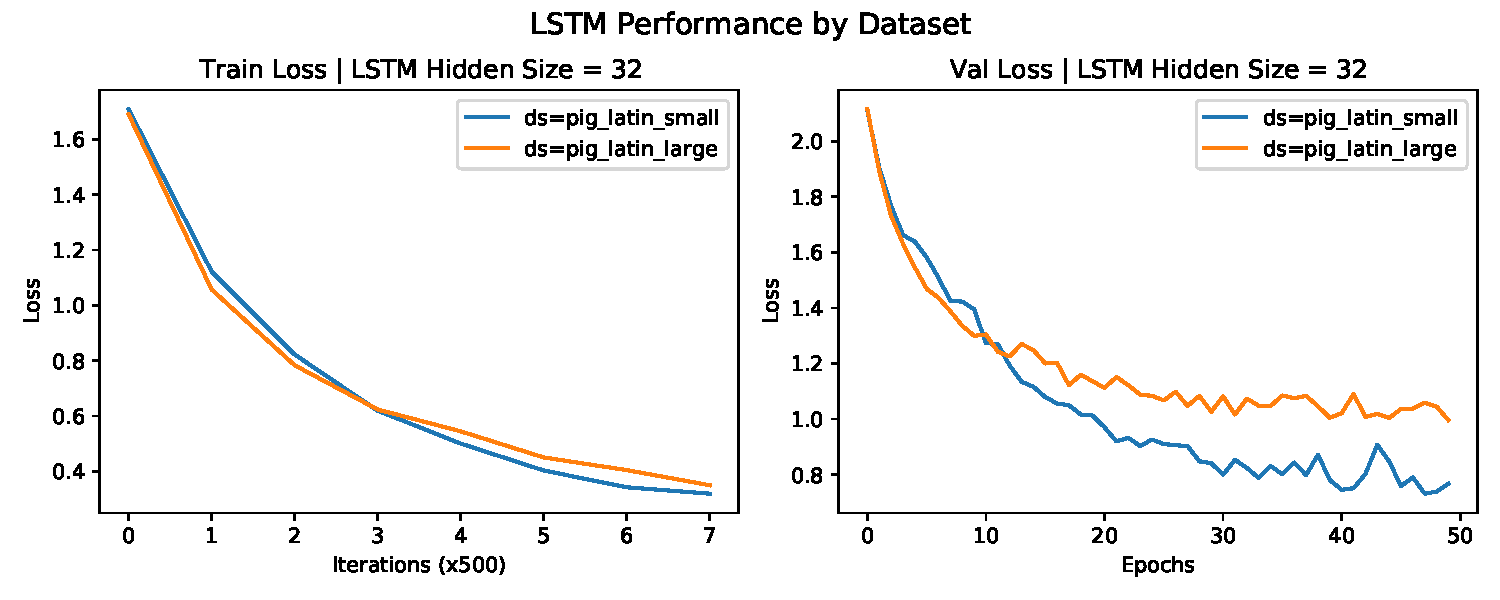
\includegraphics[width=\linewidth]{loss_plot_lstm}

\begin{quote}
... and your analysis

Does  either  model perform significantly better?  Why might this be the case?
\end{quote}

The \texttt{pig\_latin\_small} model performed better with lower validation loss because \todo{}.



\subsection*{Model Failure}

\begin{quote}
Identify a distinct failure mode and briefly describe it.
\end{quote}

\begin{lstlisting}
source:		bond-street print-shops are good-for-nothing 
translated:	ondertay-inbay inptray-ospatshay areway oodgay-orfay-othingn

ground-truth: ondbay-eetstray intpray-opsshay areway oodgay-orfay-othingnay
\end{lstlisting}

It appears that the model fails at words with hyphens. % and often fails at words that start with vowel, with which it often correctly adds ``-ay'' at the end but scrambles the other letters.


\subsection*{Model size}


\begin{quote}
Write down the number of neurons and connections of this encoder model as a function of H, K, and D.  For simplicity, you may ignore the bias units.
\end{quote}

Number of neurons: \todo{}

Number of connections: \todo{}










\end{document}
